% Title: Report LaTex File: Hardware Development
% Auther: DC Eksteen
% Student Number: 22623906
% Contact: 22623906@sun.ac.za
% Date: 2022/09/14
% Version: 2.0

\chapter{Testing Results}
\label{ch:testing}

\begin{figure}[H]
	\centering
	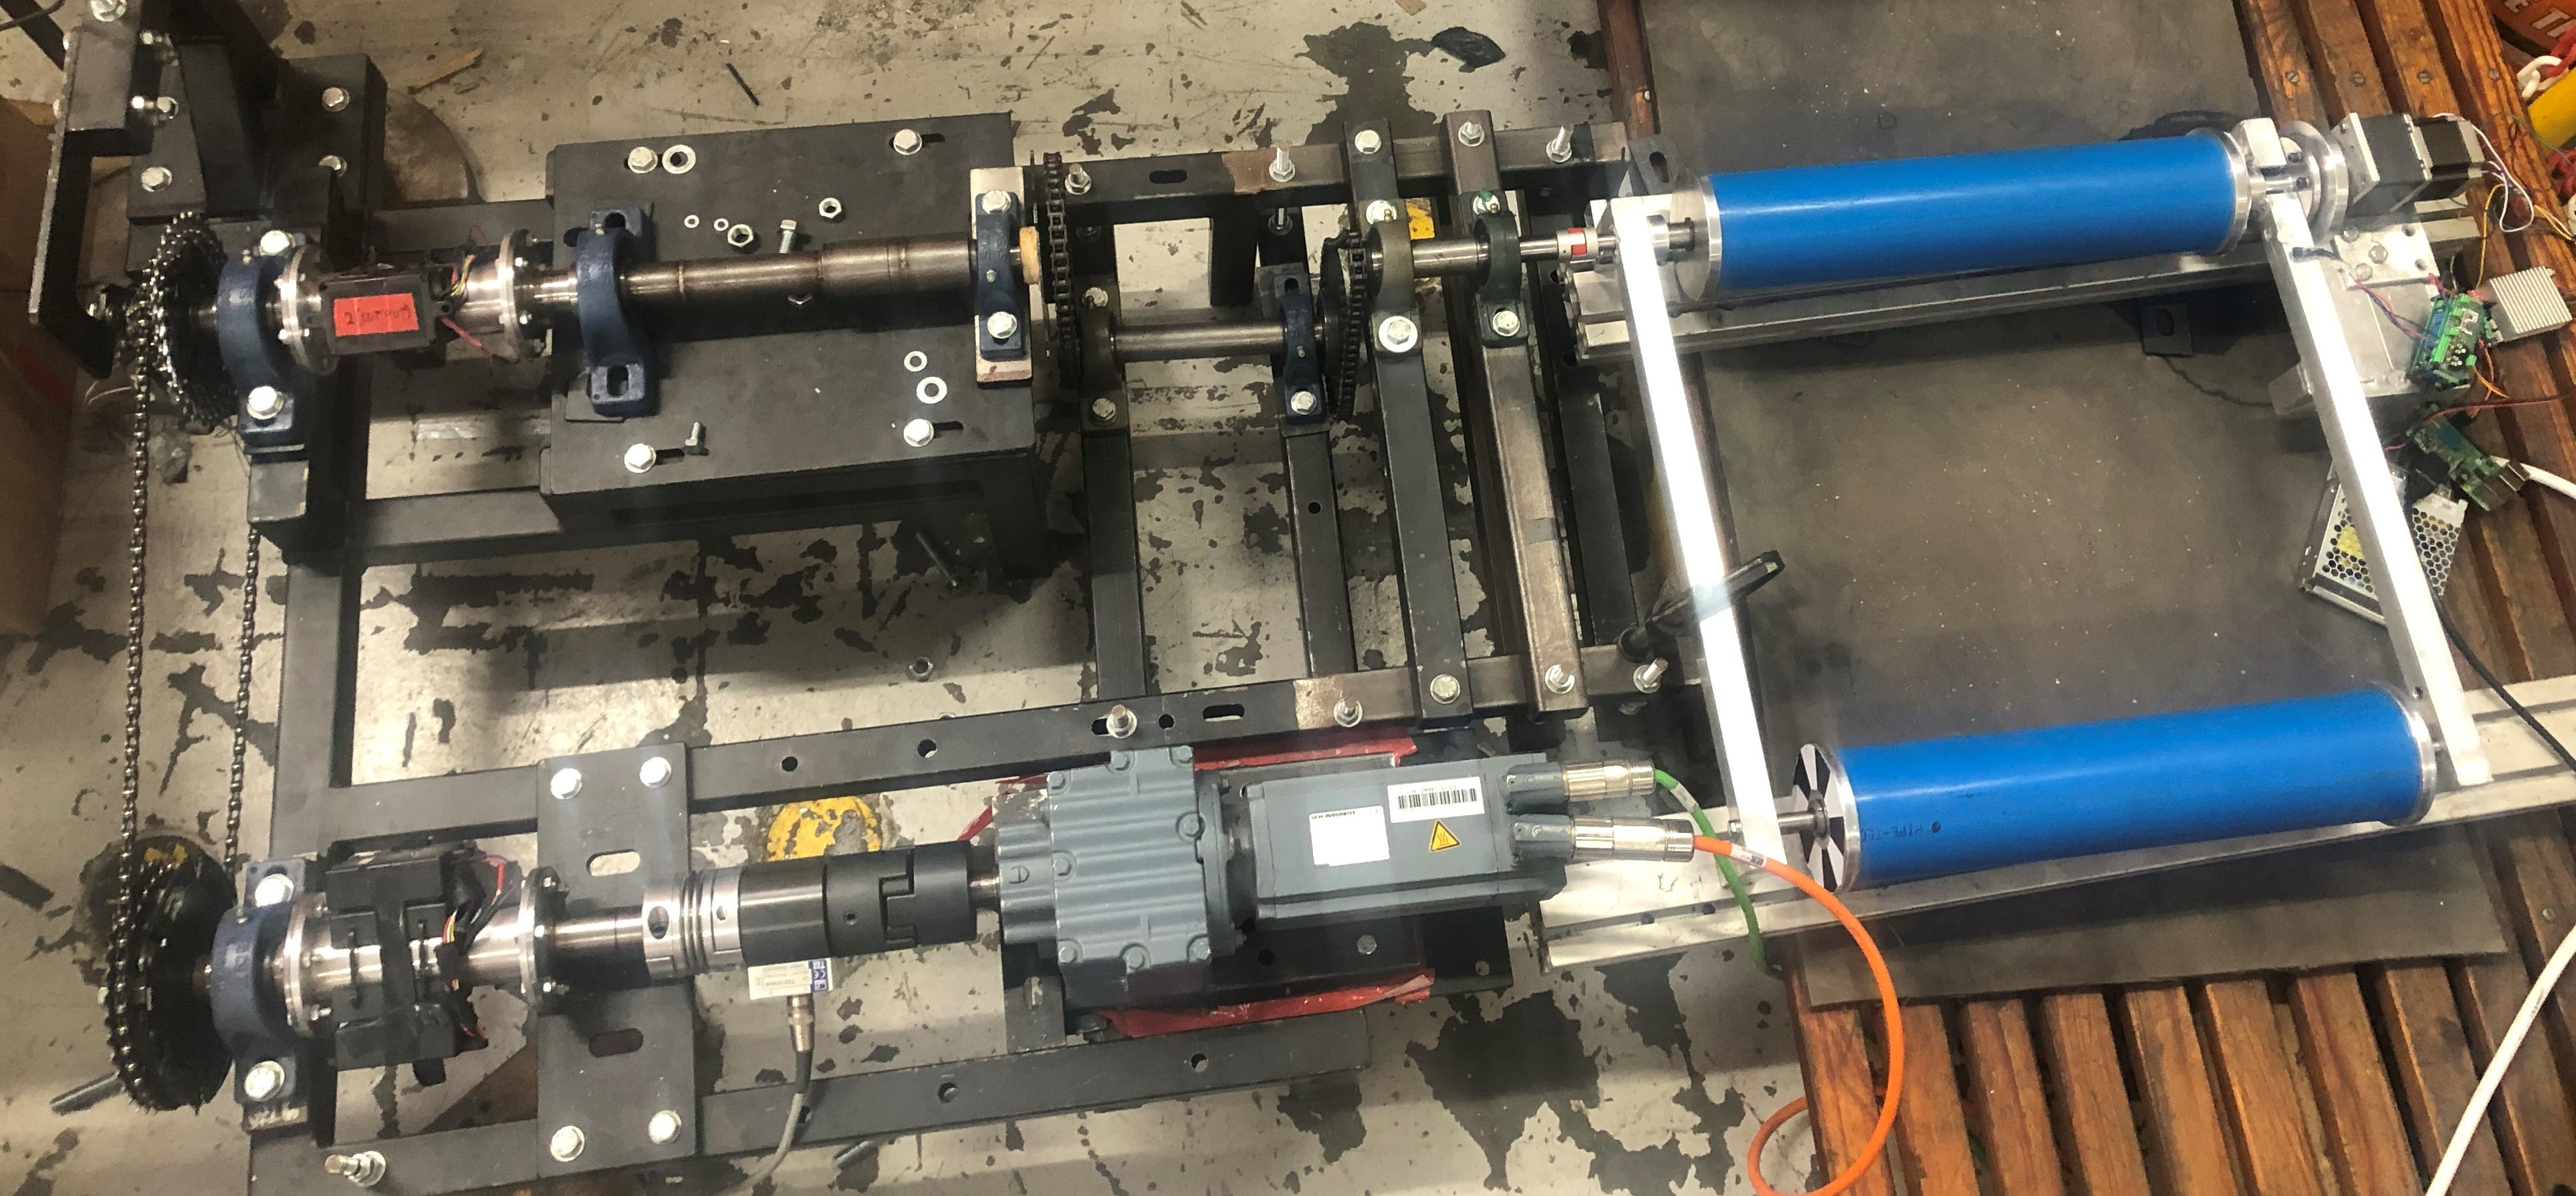
\includegraphics[width=0.5\linewidth]{TestSetup.jpg}
	\caption{Test Setup}
	\label{fig:test}
\end{figure}

Figure~\ref{fig:test} shows the setup that was used to determine the braking torque characteristics of the built eddy current brake. The setup shows a Eurodrive servo motor connected to a rotary torque transducer. The output shaft of the torque transducer is then connected to the power roller shaft of the trainer through a series of gears and chains in order to reach higher operating speeds than the motor would otherwise ba capable of reaching.

Figure~\ref{fig:testgraph} shows the torque curves that were measured at different roller speeds. Figure~\ref{fig:sensorComp} compares the measured torque curve with maximum breaking applied at various speeds with the mathematical model of the brake. 

It is clear that the mathematical model served as a good basis for designing the brake, and that acceptable results were achieved.

\begin{figure}[H]
	\centering
	\begin{subfigure}[t]{.45\textwidth}
		\centering
		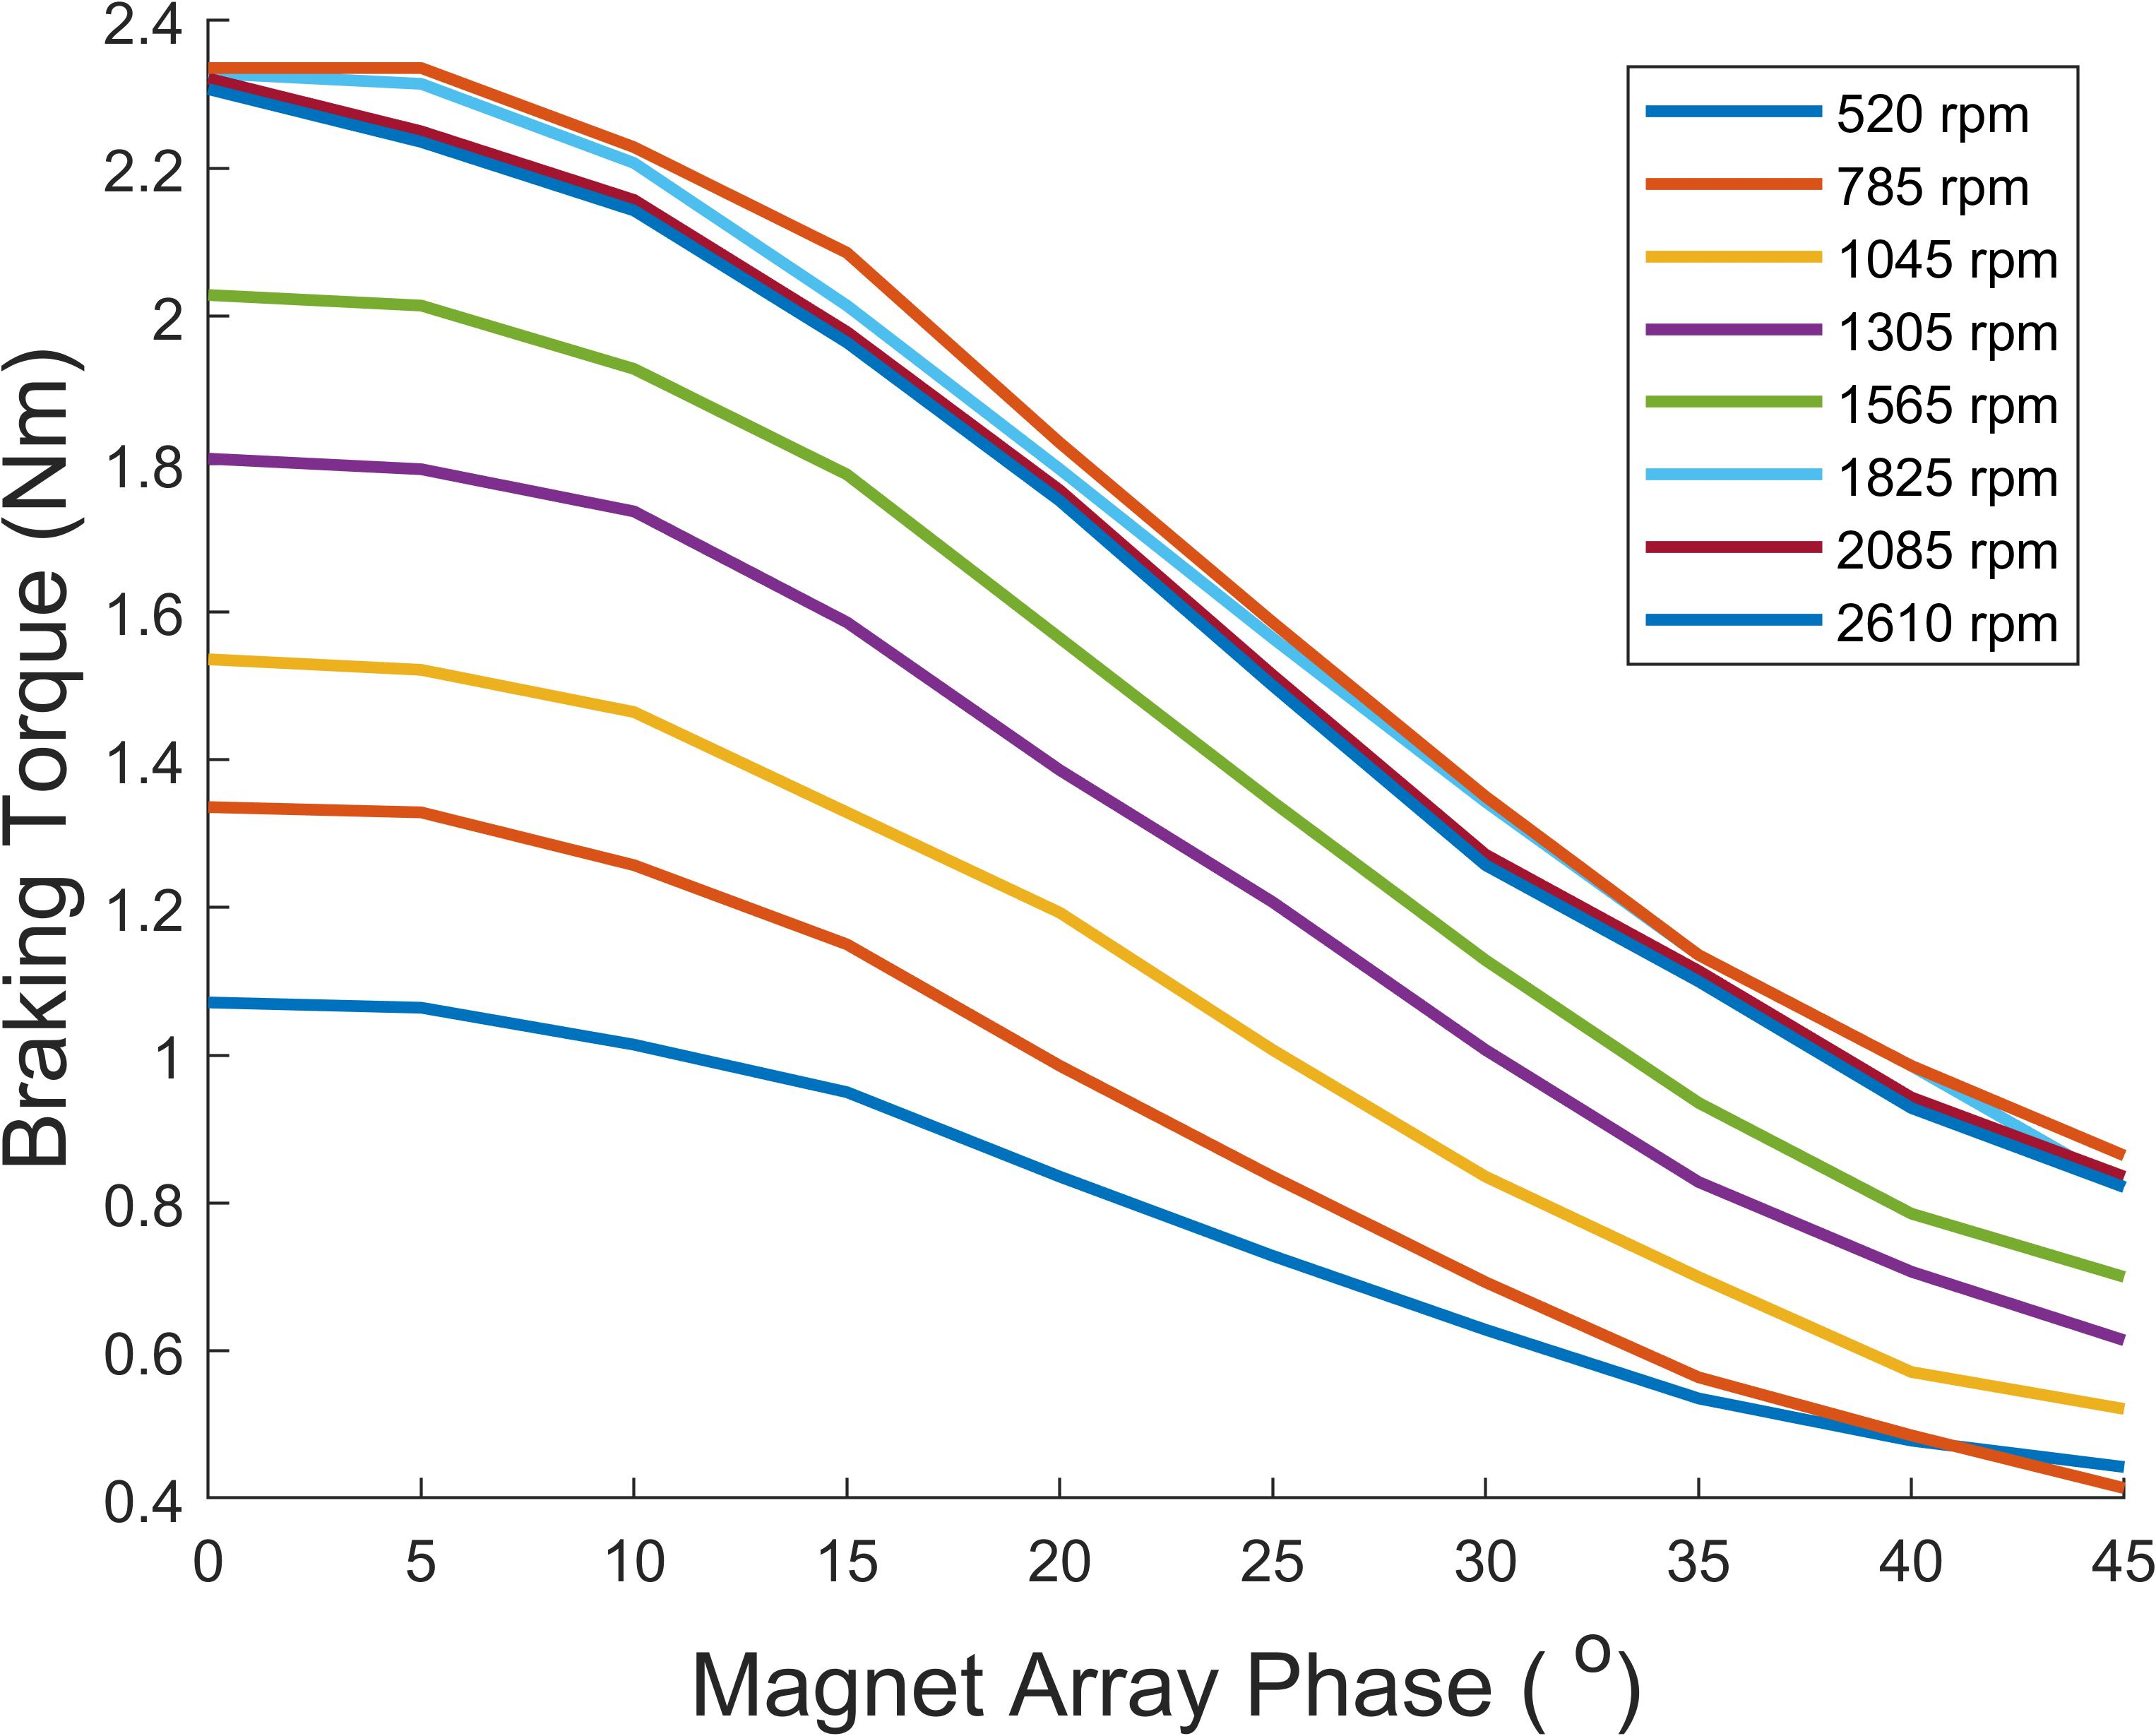
\includegraphics[width=\linewidth]{TestGraph.jpg}
		\caption{Braking Torque Curves}
		\label{fig:testgraph}
	\end{subfigure}
	\hfill
	\begin{subfigure}[t]{.45\textwidth}
		\centering
		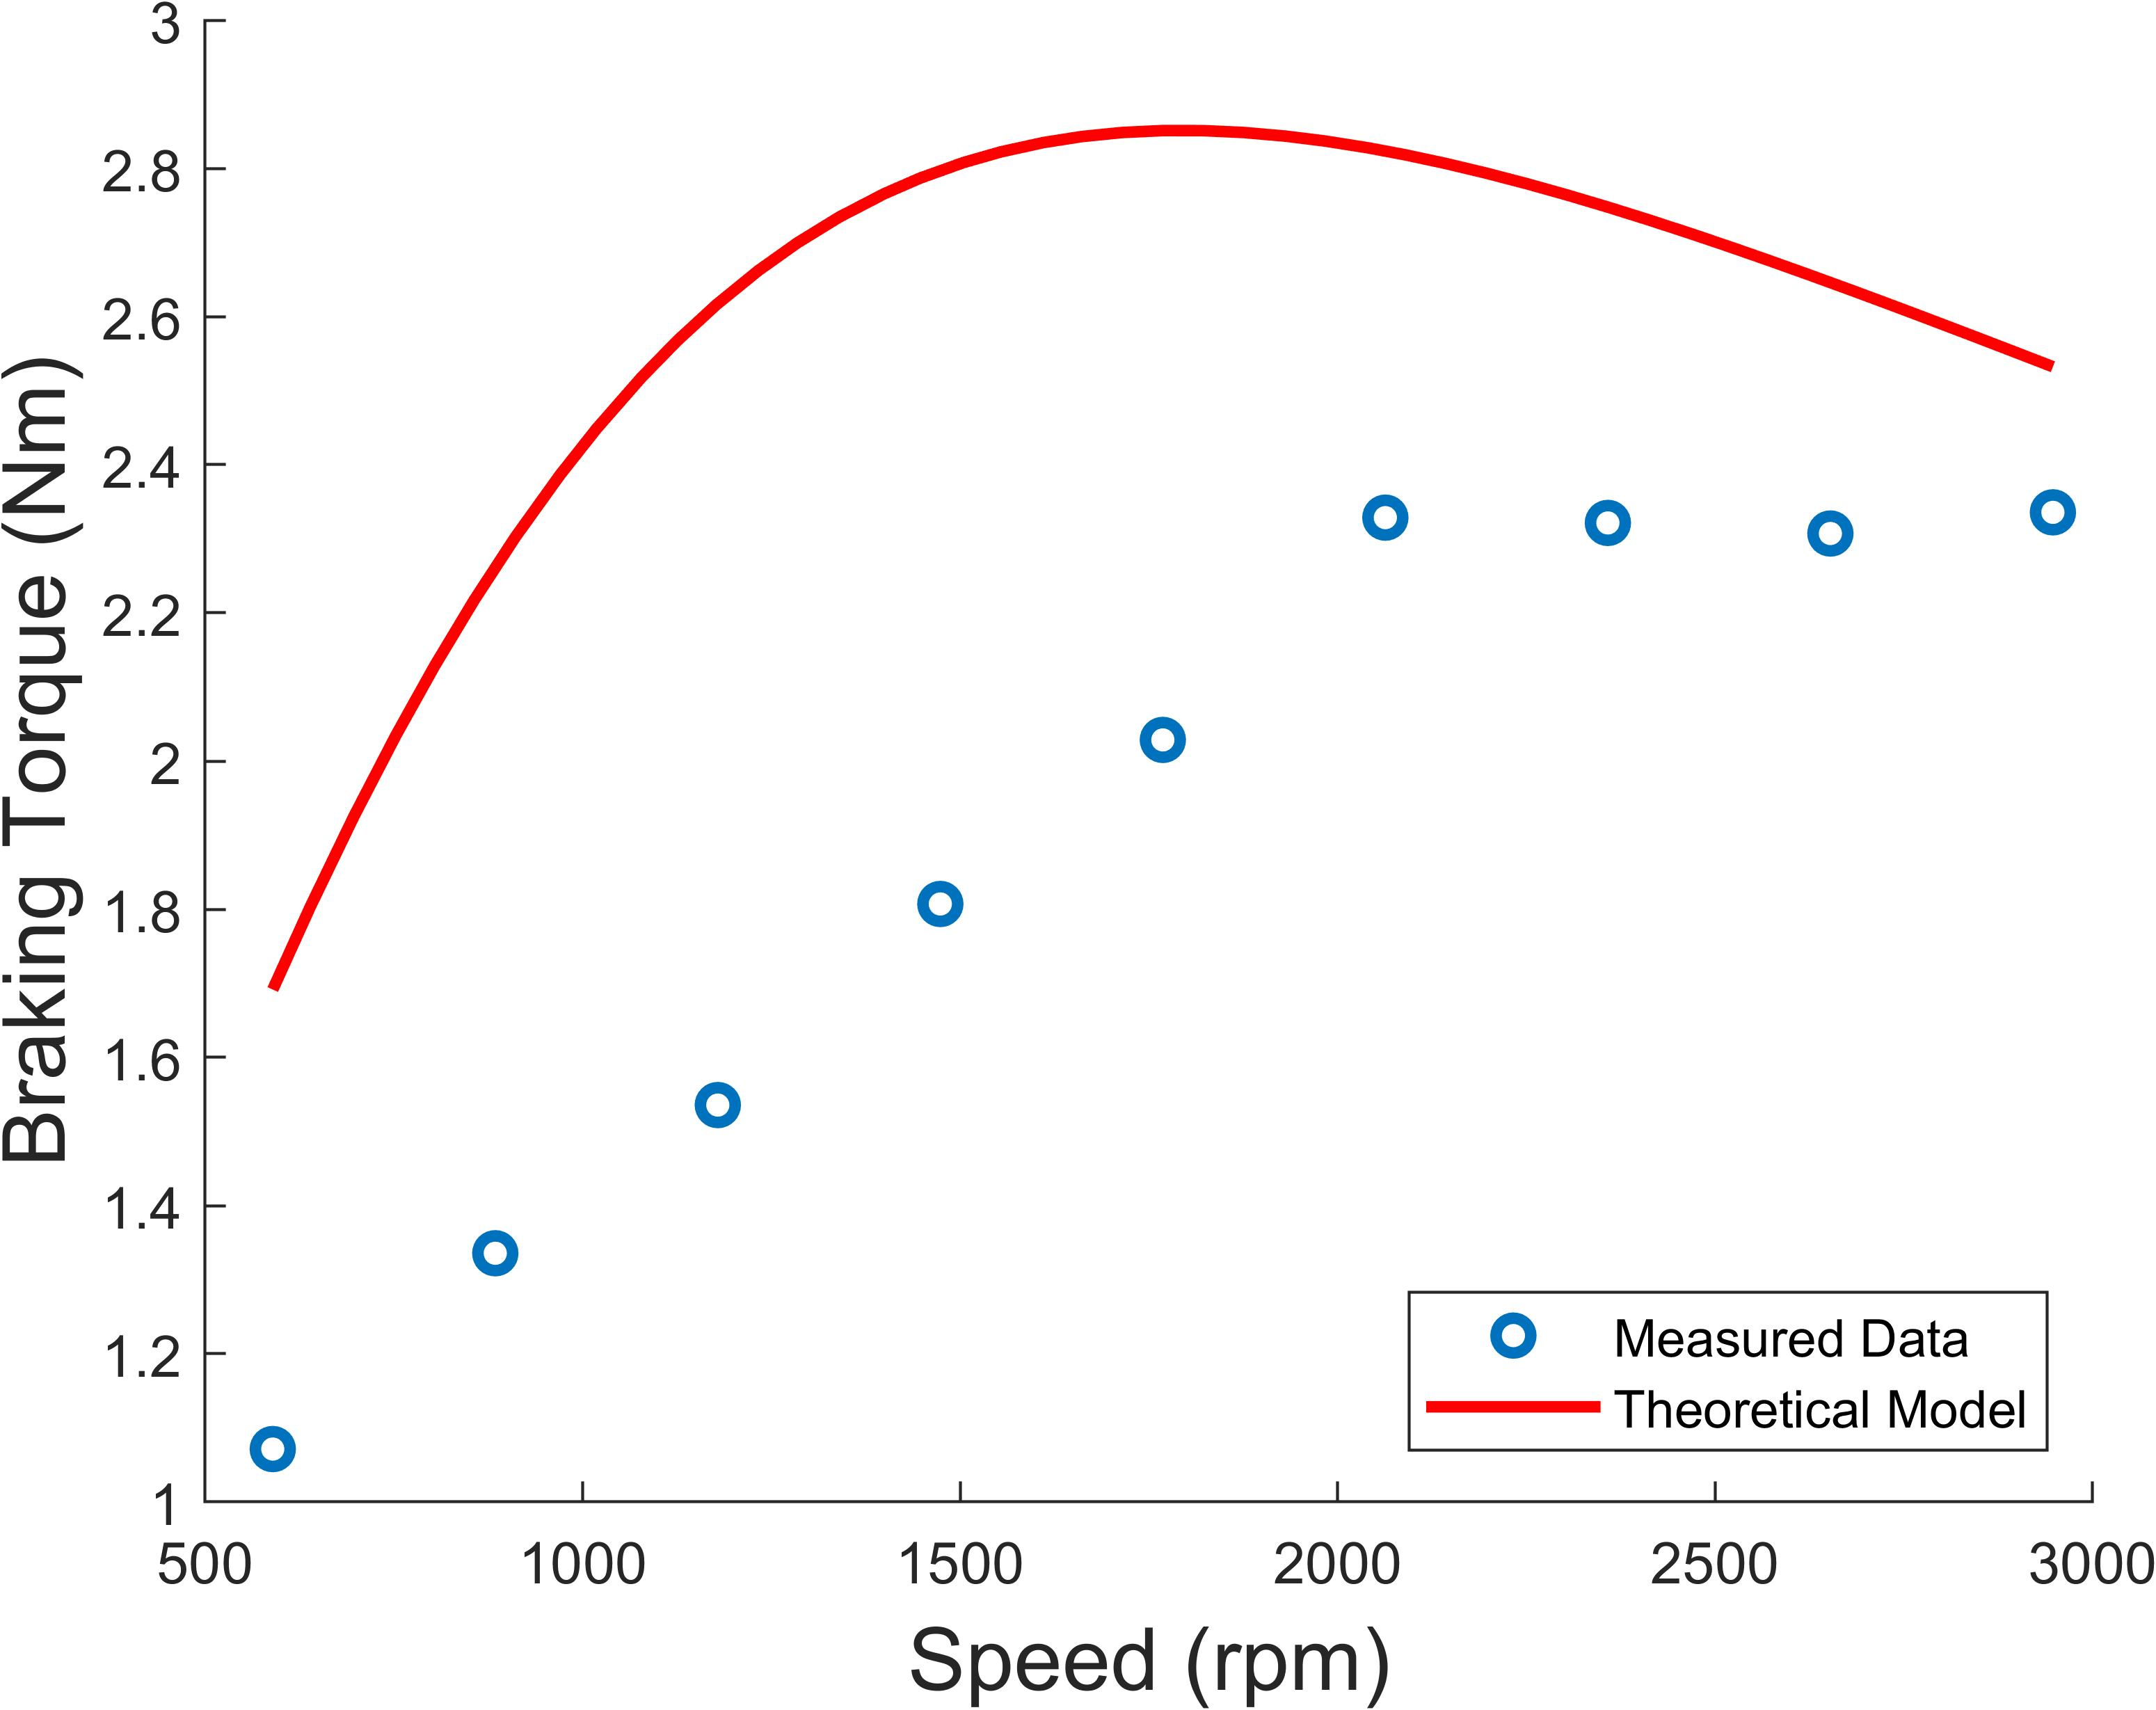
\includegraphics[width = \linewidth]{TestComp.jpg}
		\caption{Theoretical Model Comparison}
		\label{fig:sensorComp}
	\end{subfigure}
	\caption{Experimental Data}
	\label{fig:tgraph}
\end{figure}

Using the data that was gathered over multiple sets of tests, a surface plot could be fitted to a subset of the measurement data. Figure~\ref{fig:valid} shows the resulting surface plot that was found by fitting third order polynomials in both the x~and~y directions. A separate subset of data was then used to validate and refine the determined model.

\begin{figure}[H]
	\centering
	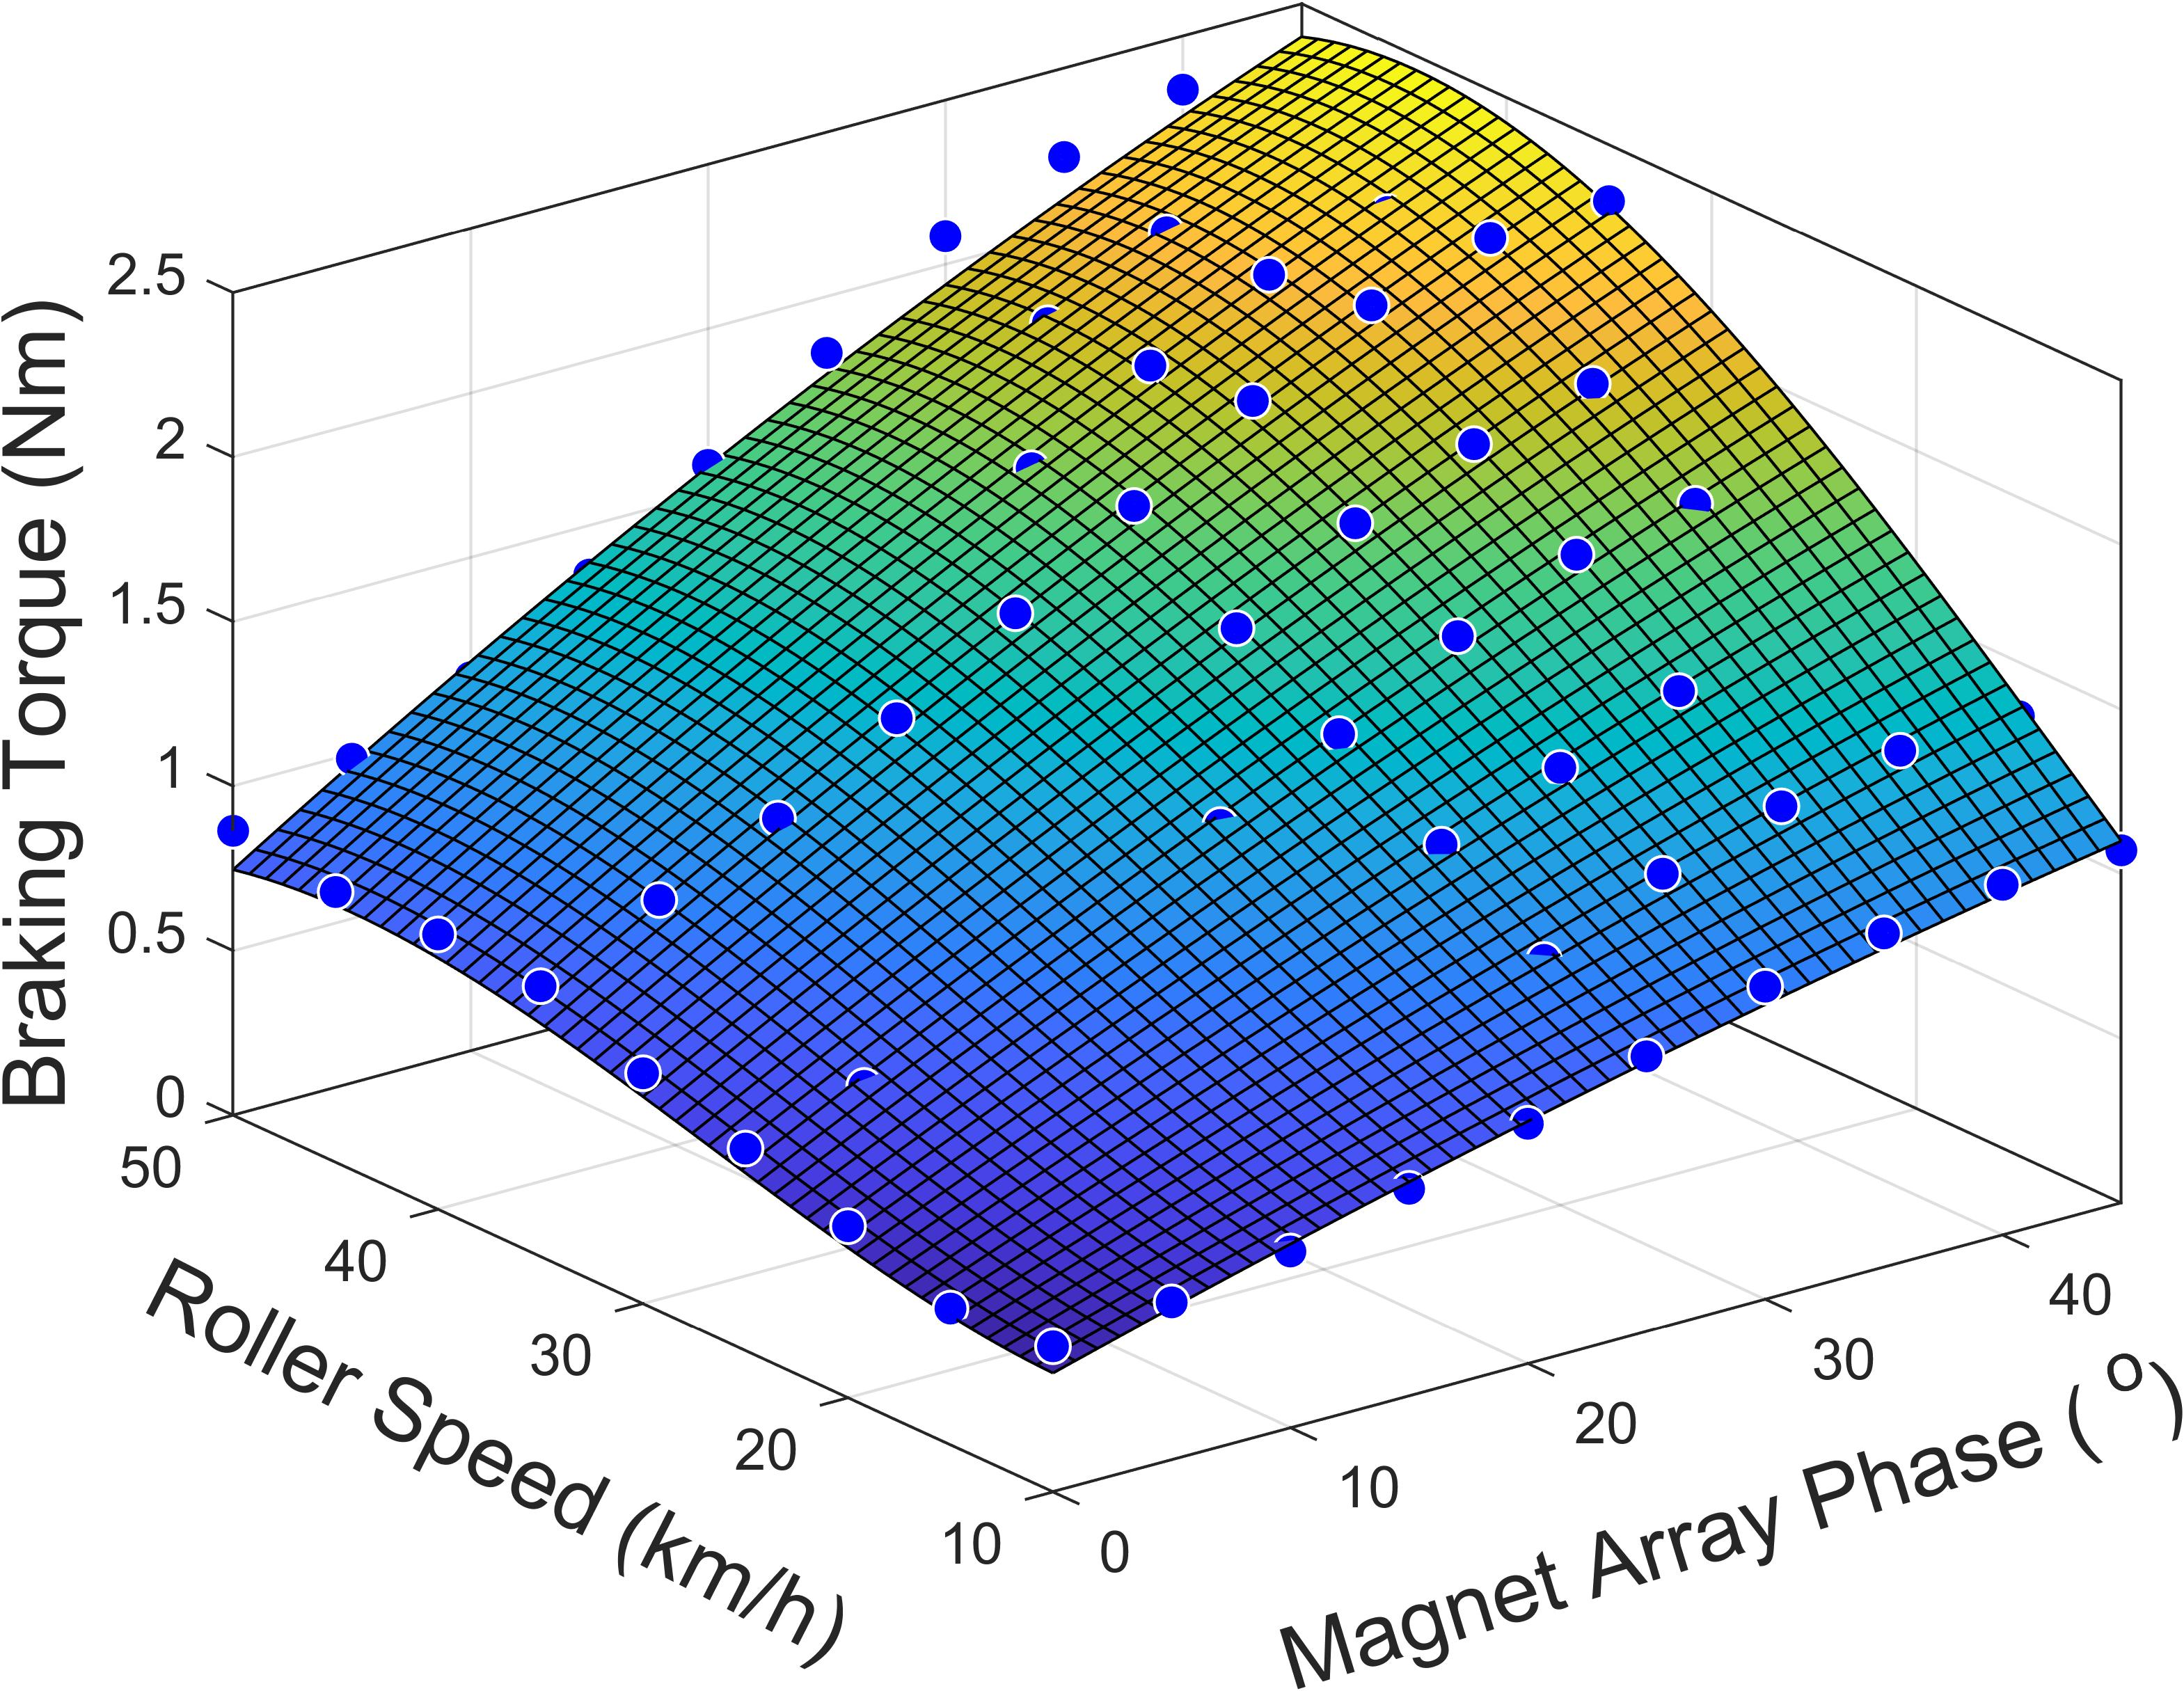
\includegraphics[width=0.6\linewidth]{Valid.jpg}
	\caption{Model Surface Plot Fit}
	\label{fig:valid}
\end{figure}